\subsection{Use cases}
Use cases beskriver hvordan en eventuel spiller interagere med spillet. 
\begin{figure}[h]
    \centering
    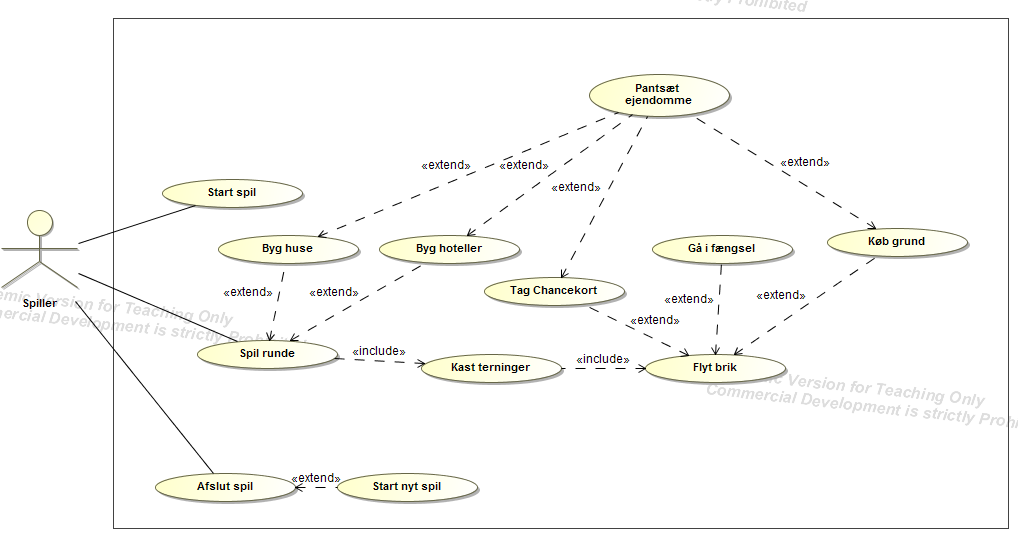
\includegraphics[width=\textwidth]{sources/5_analyse/UseCaseDiagram.PNG}
    \caption{Use case diagram}
    \label{fig:UC1}
\end{figure}

Ud fra diagrammet er der blevet udvalgt nogle kritiske use cases, som er afgørende i forhold til hvordan spillet spilles. 

\begin{itemize}
    \item Start spil
    \item Flyt brik
    \item Køb grund
    \item Gå i fængsel
    \item Tag chancekort
    \item Afslut spil
\end{itemize}

\newpage
\subsection{Use case beskrivelser}

\begin{center}
\begin{longtable}{|l|p{11cm}|}
\hline
Navn &  UC1 - Start spil\\
\hline
Short description & Spillerne starter spillet på computeren \\
\hline
Precondition & Programmet er installeret på computeren \\
\hline
Postcondition & Spillet er startet med de valgte antal spillere \\
\hline
Fejlsituationer & Ugyldigt antal spillere \\
\hline
Status i tilfælde af fejl & Spillet starter ikke \\
\hline
Aktører & Spiller \\
\hline
Udløser & Spillerne vil gerne spille spillet \\
\hline
Standard process &  
\begin{minipage}[t]{1\textwidth}
  \begin{enumerate}
      \item Spillet startes op på computeren
      \item Der vælges et antal spillere fra 2-6
      \item Der vælges navn for spillerne
      \begin{itemize}
          \item Spiller 2-6 vælger navn 
          \newline
          \emph{gentag indtil alle spiller har valgt navn}.
      \end{itemize}
      \item Der vælges farve for spillerne
      \begin{itemize}
          \item Spiller 2-6 vælger farve 
          \newline
          \emph{gentag indtil alle spiller har valgt en farve}.
      \end{itemize}
      \item Der vælges en brik til alle spillerne
      \begin{itemize}
          \item Spiller 2-6 vælger brik 
          \newline
          \emph{gentag indtil alle spiller har valgt en brik}.
      \end{itemize}
      \item Spillet starter med de valgte navne, farver og brikker.\vspace{0.5cm}
  \end{enumerate} 
  \end{minipage}
\\
\hline
Alternativ process & 
\begin{minipage}[t]{1\textwidth}
 \begin{itemize}
 \vspace{0.5cm}
     \item Der indtaster mindre eller flere spillere end 2-6
        \begin{enumerate}
            \item Spillet giver en fejlbesked
            \item Spilleren ændrer antal spillere
            \item forsætter fra 2. i hoveddelen
        \end{enumerate}
    \item Der vælges en forkert brik, eller en brik der er optaget
    \begin{enumerate}
        \item Spillet giver en fejlbesked
        \item Spilleren vælger en anden brik
        \item fortsætter fra 7. i hoveddelen
    \end{enumerate}
 \end{itemize}
\end{minipage}

\\
\hline
\end{longtable}
\end{center}



\begin{center}
\begin{longtable}{|l|p{11cm}|}
\hline
Navn &  UC2 - Flyt brik\\
\hline
Short description & Den nuværende spiller kaster terningerne og flytter sin brik \\
\hline
Precondition & Det er spillerens tur \\
\hline
Postcondition & Spilleren har taget sin tur, og turen er gået videre til den næste spiller \\
\hline
Fejlsituationer & Ingen \\
\hline
Status i tilfælde af fejl & Spilleren tager ikke sin tur \\
\hline
Aktører & Spiller \\
\hline
Udløser & Det er spillerens tur \\
\hline
Standard process &  
\begin{minipage}[t]{1\textwidth}
  \begin{enumerate}
      \item Spilleren kaster terningerne.
      \item Spilleren flytter sin brik fra det nuværende felt \newline til det næste felt.
      \begin{itemize}
          \item Spilleren lander på en grund.\newline
          \emph{Se alternativ process.} 
          \item Spilleren lander på besøg i fængsel.\newline
          \emph{Se alternativ process.}
          \item Spilleren lander på gå i fængsel.\newline
          \emph{Se alternativ process.}
          \item Spilleren lander på Prøv lykken.\newline
          \emph{Se alternativ process.}
          \item Spilleren lander på Parkering.\newline
          \emph{Se alternativ process.}
          \item Spilleren lander på et beskatningsfelt.\newline
          \emph{Se alternativ process.}
      \end{itemize}
      \item Passerede spilleren start?
      \begin{itemize}
          \item Modtag 4000. 
      \end{itemize}
      \item Slog spilleren to ens?
      \begin{itemize}
          \item Gå til trin 1.
      \end{itemize}
      \item Turen går videre til den næste spiller.\vspace{0.5cm}
  \end{enumerate} 
  \end{minipage}
\\
\hline
Alternativ process & 
\begin{minipage}[t]{1\textwidth}
 \begin{itemize}
     \item Grund
     \begin{enumerate}
         \item Hvis ingen ejer grunden,\newline vil spilleren købe grunden? (Se UC3)
         \item Hvis en anden spiller ejer grunden, betal leje.
         \item Hvis spilleren selv ejer grunden, ingenting. \newline (Gå til trin 3. i hoveddel)
     \end{enumerate}
     \item Besøg i fængsel
     \begin{enumerate}
         \item Der sker ingenting
         \item Gå til trin 3. i hoveddel.
     \end{enumerate}
     \item Gå i fængsel
     \begin{enumerate}
         \item Flyt spillerens brik i fængsel
         \item Gå til trin 5. i hoveddel.
     \end{enumerate}
     \item Prøv lykken
     \begin{enumerate}
         \item Tag chancekort 
         \item udfør chancekort.
         \item Gå til trin 3. i hoveddel.
     \end{enumerate}
     \item Parkering
     \begin{enumerate}
         \item Gå til trin 3. i hoveddel.
     \end{enumerate}
     \item Beskatningsfelt
     \begin{enumerate}
         \item Betal skat
         \item Gå til trin 3. i hoveddel.
     \end{enumerate}
 \end{itemize}
\end{minipage}

\\
\hline
\end{longtable}
\end{center}